\documentclass{beamer}

\usepackage[ngerman]{babel}
\usepackage{graphicx} % fuer Bilder
\usepackage{listings} % fuer Code

\usetheme{Goettingen}

\lstset{language=C++} % fuer c++ code style

\title{Prozesslenkung: Hierarchische Zustandsautomaten II}
\subtitle{Implementierung Hierarchischer Zustandsautomaten}
\author{Katja Kirstein, Anne-Lena Kowalka, Marian Triebe, Eugen Winter}
\date{\today} 

\begin{document}
\begin{frame}
\titlepage
\end{frame}

%% Themen uebersicht
\begin{frame}
 \frametitle{Themen}
 \begin{itemize}
  \item Grundlagen GoF
  \item Externe Statevariablen
  \item Guards/Choice Points
  \item Entry und Exit Code
  \item History
  \item Timer
 \end{itemize}
\end{frame}

%% GoF fsm Beispiel (Klassendiagramm)
\begin{frame}
 \frametitle{GoF State Pattern Struktur}
 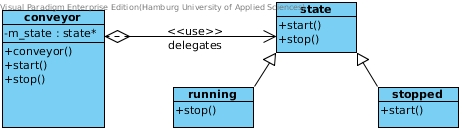
\includegraphics[scale=.6]{img/fsm_gof.jpg}
 \begin{itemize}
  \item Kontext-Klasse (conveyor)
  \item Zustands Basisklasse (state)
  \item Zust\"ande (running, stopped)
 \end{itemize}
\end{frame}

%% Grundlagen GoF
\begin{frame}
 \frametitle{Grundlagen GoF}
 Die klassiche GoF Implementierung hat einige schw\"achen
 \begin{itemize}
  \item Hoher Speicherverbrauch, da jeder Zustand im Speicher gehalten werden muss, auch wenn diese eigentlich nicht verwendet werden
  \item Der h\"ohere Speicherverbrauch kann allerdings mit dem Placement New Operator umgangen werden
  \item Kontext muss eventuell immer mit \"ubergeben werden
 \end{itemize}
\end{frame}

%% GoF fsm Systemgrenzen
\begin{frame}
 \frametitle{Systemgrenzen}
 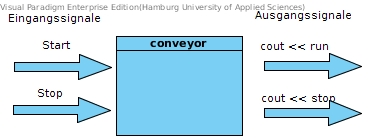
\includegraphics[scale=.7]{img/Systemgrenzen_fsm_gof.jpg}
\end{frame}

%% GoF fsm Automat
\begin{frame}
 \frametitle{Automat}
\end{frame}

%% GoF fsm States in Code I
\begin{frame}
 \frametitle{GoF States in Code I}
 \begin{itemize}
  \item Alle States erben von einer Oberstate Klasse
  \item Der Oberstate implementiert alle Events aller Zust\"ande als leere virtuelle Funktion
  \item Der jeweilige Zustand implementiert nur seine eigenen Events, nicht relevante
  Events werden an die leeren Methoden der Basisklasse weitergereicht
 \end{itemize}
\end{frame}

%% GoF fsm States in Code (Header)
\begin{frame}[fragile]
 \frametitle{GoF States in Code (Header)}
 \begin{lstlisting}
  struct state {
    virtual ~state() { }
    virtual void start() { }
    virtual void stop() { }
  };

  struct running : public state {
    void stop();
  };

  struct stopped : public state {
    void start();
  };
 \end{lstlisting}
\end{frame}

%% GoF fsm States in Code (Implementierung/CPP)
\begin{frame}[fragile]
 \frametitle{GoF States in Code (Implementierung)}
 \begin{lstlisting}
  // transition running -> stopped
  void running::stop() {
    new (this) stopped;
    cout << "stop() / stop" << endl;
  }

  // transition stopped -> running
  void stopped::start() {
    new (this) running;
    cout << "start() / run" << endl;
  }
 \end{lstlisting}
\end{frame}

%% GoF fsm Kontext Klasse
\begin{frame}
 \frametitle{GoF Kontext Klasse}
 \begin{itemize}
  \item Sicht von au{\ss}en auf die FSM
  \item Dient als Delegator zu den Zust\"anden
  \item Bedient alle Eingangssignale durch Funktionen
 \end{itemize}
\end{frame}

%% GoF fsm Konext Klasse
\begin{frame}[fragile]
 \frametitle{GoF Kontext Klasse in Code}
 Header:
 \begin{lstlisting}
  struct conveyor {
    conveyor() : m_state(new stopped) { }
    ~conveyor() { delete m_state; }
    void start();
    void stop();
   private:
    state* m_state;
  };
 \end{lstlisting}
 Implementierung:
 \begin{lstlisting}
  void conveyor::start() {
    m_state->start();
  }
  void conveyor::stop() {
    m_state->stop();
  }
 \end{lstlisting}
\end{frame}

%% Schritte zum erstellen einer FSM
\begin{frame}
 \frametitle{Schritte zum erstellen einer FSM}
 \begin{enumerate}
  \item Erstellen der Systemgrenzen
  \item Erstellen einer FSM
  \item Umwandlung in Code
  \begin{itemize}
   \item Kontextklasse, Funktionsnamen als Eingangssignale
   \item Basisklasse f\"ur Zust\"ande erstellen
   \item Zustandsklassen erben von der Basisklasse und implementieren nur die eigenen Reaktionen neu
  \end{itemize}
  \item Pr\"ufen ob Code und Systemgrenzen/Diagramm zusammenpassen
  \begin{itemize}
   \item Sind alle Eingangssignale als Funktionen zu finden?
   \item Werden alle Ausgangssignale verwendet/ausgegeben?
   \item Die Namen f\"ur Eingangssignale/Ausgangssignale sollten konsistent sein, da Fehler sonst vorprogrammiert!
  \end{itemize}
 \end{enumerate}
\end{frame}

%% Übung GoF
\begin{frame}
 \frametitle{\"Ubung Lichtschalter}
 Erstellt die Systemgrenzen, Automatendiagramm, und Code eines Lichtschalters (An und Aus Button). (15 Min)
\end{frame}

%% Externe Statevariablen
\begin{frame}
 \frametitle{Externe Statevariablen}
  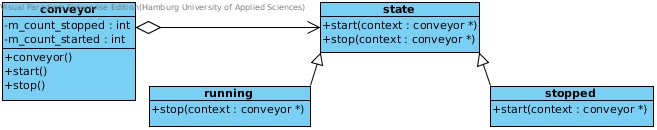
\includegraphics[scale=.44]{img/fsm_externe_state_var.jpg}
\end{frame}

%% Implementierung von externen Statevariablen I
\begin{frame}[fragile]
 \frametitle{Implementierung von externen Statevariablen I}
 \begin{lstlisting}
struct conveyor {
  friend struct running;
  friend struct stopped;
  conveyor()
      : m_state(new stopped),
        m_count_stopped(0),
        m_count_started(0) { }
  ~conveyor() { delete m_state; }
  void start();
  void stop();
 private:
  state* m_state;
  int m_count_stopped;
  int m_count_started;
};
\end{lstlisting}
\end{frame}

%% Implementierung von externen Statevariablen II
\begin{frame}[fragile]
  \frametitle{Implementierung von externen Statevariablen II}
  Header:
  \begin{lstlisting}
struct state {
  virtual ~state() { }
  virtual void start(conveyor* context) { }
  virtual void stop(conveyor* context) { }
};

struct running : public state {
  void stop(conveyor* context);
};

struct stopped : public state {
  void start(conveyor* context);
};
  \end{lstlisting}

\end{frame}


%% Implementierung von externen Statevariablen III
\begin{frame}[fragile]
  \frametitle{Implementierung von externen Statevariablen III}
  Implementierung:
  \begin{lstlisting}
// transition running -> stopped
void running::stop(conveyor* context) {
  ++context->m_count_stopped;
  new (this) stopped;
}
// transition stopped -> running
void stopped::start(conveyor* context) {
  ++context->m_count_started;
  new (this) running;
}
void conveyor::start() {
  m_state->start(this);
}
void conveyor::stop() {
  m_state->stop(this);
}
  \end{lstlisting}

\end{frame}

%% Guards
\begin{frame}
 \frametitle{Guards}
 Guard Automat:
\end{frame}

%% Guard Implementierung
\begin{frame}[fragile]
 \frametitle{Guards Implementierung}
 Implementierung:
  \begin{lstlisting}
// transition stopped -> running
void stopped::start(conveyor* context) {
  ++context->m_count_started;
  if (context->m_count_started <= 2) {
    new (this) running;
  } else {
    return;
  }
}
  \end{lstlisting}
\end{frame}

%% Choice Points
\begin{frame}
 \frametitle{Choice Points}
\end{frame}

%% Übung Guards
\begin{frame}
 \frametitle{\"Ubung Lichtschalter II}
\end{frame}

%% Entry/Exit Code 1
\begin{frame}
	\frametitle{Entry/Exit Code in HSM }
	\begin{itemize}
		\item Zustandswechsel d\"urfen Hierarchieebenen nicht \"uberspringen
		\item exit() wird durchgef\"uhrt, wenn Signale in der Hierarchie "nach oben" weitergereicht werden 
		\item entry() wird  durchgef\"uhrt, wenn Signale in der Hierarchie "nach unten" weitergereicht werden
	\end{itemize}
\end{frame}

%% Entry/Exit Code 2
\begin{frame}
	\frametitle{Entry/Exit Code in HSM }
	\begin{itemize}
		\item Beispiel exit: State S12 erh\"alt Signal e
	\end{itemize}
	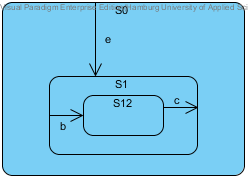
\includegraphics[scale=.6]{img/beispiel_exitSM}
\end{frame}

%% Exit Code 3
\begin{frame}[fragile]
	\frametitle{Entry/Exit Code in HSM }
	\begin{lstlisting}
	//State S12 erhaelt Signal e
    void StateS12::sigE() {
        exit(); 
        new (this) StateS1;
        sigE();
	}
	\end{lstlisting}
	\begin{itemize}
		\item die exit-Funktion ist in jedem Zustand definiert
		\item wenn auch der Top-Zustand nicht auf ein Signal reagiert, sollte dieser z.B. eine
		failure-Methode haben, um den Fehler anzuzeigen
	\end{itemize}
\end{frame}

%% Entry Code 1
\begin{frame}
	\frametitle{Entry/Exit Code in HSM  }
	\begin{itemize}
		\item Beispiel entry: State S1 erh\"alt Signal b
	\end{itemize}
	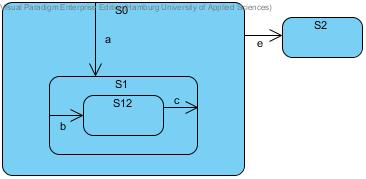
\includegraphics[scale=.6]{img/beispiel_entrySM}
\end{frame}

%% Entry Code 2
\begin{frame}[fragile]
	\frametitle{Entry/Exit Code in HSM }
	\begin{lstlisting}
	//State S1 erhaelt Signal b
    void StateS1::init(T* t){
    //t ist ein Pointer auf die Kontextklasse
        void* history = 
        t->getStateFromHistory(StateS1ID);
        if(history != 0){
	        memcpy(this, &history, 4);
        }
        else{
            new (this) StateS12;
            entry();
        }
    init(); 
    }
	\end{lstlisting}
\end{frame}

%% Entry Code 3
\begin{frame}[fragile]
	\begin{itemize}
		\item die entry-Funktion ist in jedem Zustand definiert
		\item init() f\"uhrt dazu, dass -sofern ein Substate bereits in der History vorliegt- dieser direkt betreten wird; ansonsten wird er neu erzeugt
		\item der erneute init()-Aufruf darf in der vorletzten bzw. letzten Hierarchie-Ebene nicht stattfinden (ansonsten Endlosschleife) ????????? korrekt??

	\end{itemize}
\end{frame}

%% History 1
\begin{frame}
	\frametitle{History}
	\begin{itemize}
		\item Implementierung der flachen History
		\item die history-Funktion  wird in der exit-Funktion aufgerufen
		\item die Kontextklasse h\"alt ein History- Array,
		 in dem sich die Subzust\"ande mittels history-Aufruf eintragen (Index-Zuordnung z.B. \"uber enums)
	\end{itemize}
\end{frame}

%% History 2
\begin{frame}[fragile]
	\frametitle{History}
	\begin{itemize}
		\item Beispiel: S1 tr\"agt sich in History-Tabelle ein
	\end{itemize}
	\begin{lstlisting}
//StateS1 history-Funktion
voidS StateS1::history(T* t){
    //t ist ein Pointer auf die Kontextklasse
    t->
    setHistory(State::StateID::StateS1_ID,
    this);
}
	\end{lstlisting}
	\begin{itemize}
		\item der Parameter StateS1ID gibt den Index in der History-Tabelle in der Kontextklasse an
	\end{itemize}
\end{frame}

%% History 3
\begin{frame}[fragile]
	\frametitle{History}
	\begin{itemize}
		\item setHistory in der Kontextklasse:
	\end{itemize}
	\begin{lstlisting}
    void setHistory(int ID, State* ptr){
        history_[ID] = *((void**) ptr);
    }
	\end{lstlisting}
	\begin{itemize}
		\item ptr wird zu\"achst auf void** gecastet, damit man mit einer weiteren Dereferenzierung * an die virtuelle Funktionstabelle des Zustands gelangt 
	\end{itemize}
\end{frame}

%% History 4
\begin{frame}[fragile]
	\frametitle{History}
	\begin{itemize}
		\item getStateFromHistory in der Kontextklasse:
	\end{itemize}
	\begin{lstlisting}
    void* getStateFromHistory(int ID){
        return history_[ID];
    }
	\end{lstlisting}
	\begin{itemize}
		\item \"uber seine ID kann der Zustand sich seine History -sofern eine vorliegt- aus der History-Tabelle in der Kontextklasse holen
	\end{itemize}
\end{frame}


%% Timer
\begin{frame}
 \frametitle{Timer}
\end{frame}

\end{document}